\documentclass[a4paper, 12pt]{article}

\usepackage[utf8]{inputenc}
\usepackage[ngerman]{babel}
\usepackage[T1]{fontenc}

\usepackage[top = 2.85cm, bottom = 2.5cm, left = 2.5cm, right = 2.5cm]{geometry}

\usepackage{fancyhdr}
\pagestyle{fancy}
\fancyhf{}% Alle Felder loeschen
\renewcommand{\headrulewidth}{0.4pt} %obere Trennlinie
\renewcommand{\footrulewidth}{0.4pt} %obere Trennlinie
\fancyhead[R]{\today}
\fancyhead[L]{Florian Hofmann}
\fancyhead[C]{Gitarre für Anfänger}
\fancyfoot[C]{\thepage}

\usepackage{fontspec}
\setmainfont{Latin Modern Sans}

\usepackage{tabularx}
\usepackage{graphicx}
\usepackage{xcolor}
\usepackage{enumitem}
\usepackage{xspace}

\usepackage[absolute]{textpos}

\usepackage[
    bookmarks=true,
    unicode=false,
    pdftoolbar=true,
    pdfmenubar=true,
    pdfnewwindow=true,
    colorlinks=true,
    linkcolor=black,
    citecolor=green,
    filecolor=magenta,
    urlcolor=cyan!75!blue!50
]{hyperref}

% defining custom commands
\definecolor{col_ref}{gray}{0.4} % 1 = white; 0 = black
\newcounter{figurecounter}
\newcounter{referencecounter}
\newcommand{\addImage}[5]{%
    \begin{figure} [#1]
        \centering
        % Add the hypertarget above the picture to see the picture after the click
        {\color{white}\tiny \hypertarget{#5}{}}
        \includegraphics[#2]{#3}
        \caption{#4} \label{#5lbl}
    \end{figure}}

\newcommand{\figref}[1]{\setcounterref{figurecounter}{#1lbl}\hyperlink{#1}{\color{col_ref}\textsl{Abbildung \thefigurecounter}}}
\newcommand{\quotes}[1]{\glqq #1\grqq\xspace}

\pagenumbering{arabic}

\title{\Huge \textbf{Gitarre für Anfänger}}
\author{Florian Hofmann}
\date{\today}

\begin{document}
    \pagenumbering{gobble}
    \maketitle
    \tableofcontents
    \begin{textblock*}{\paperwidth}(0cm, 15cm)
    \vfill
    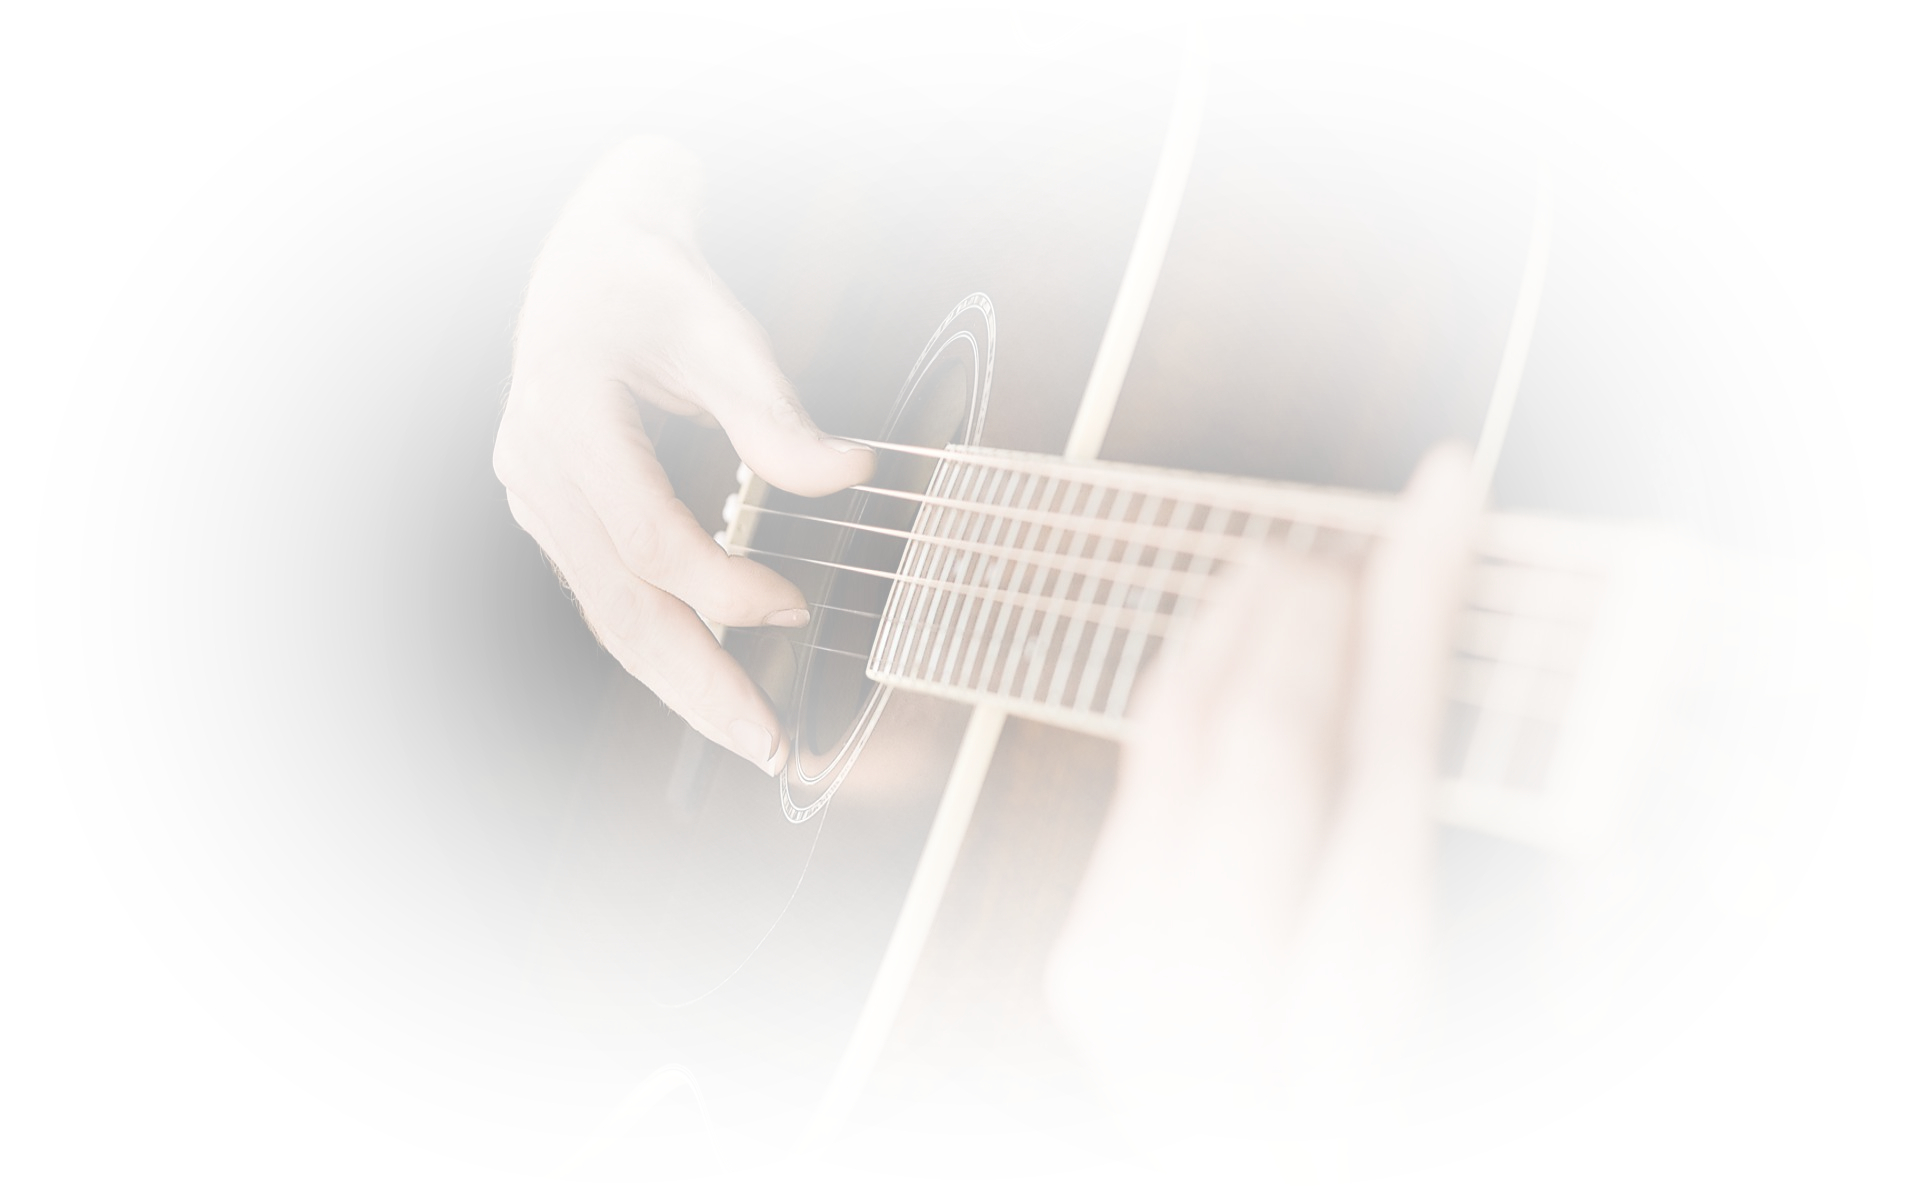
\includegraphics[width=\paperwidth]{pictures/background3}
    \end{textblock*}
    \newpage
    \pagenumbering{arabic}
    \setcounter{page}{1}
    \section{Die Gitarre}
    Zum Einstieg sollen im nachfolgenden Kapitel alle Punkte geklärt werden, die für einen
    grundlegendes Verständnis der Gitarre notwendig sind.

    \subsection{Verschiedene Gitarren}
    Es gibt die verschiedensten Arten von Gitarren. In dieser Anleitung wird vorerst allerdings nur auf Techniken der Konzertgitarre (\figref{fig:aufbau}) eingegangen.
    Nichts desto trotz sollen exemplarisch einige andere Gitarrentypen gezeigt werden. \vspace{0.25cm}\\
    \begin{tabularx}{\textwidth}{*{4}{>{\centering\arraybackslash}X}}
    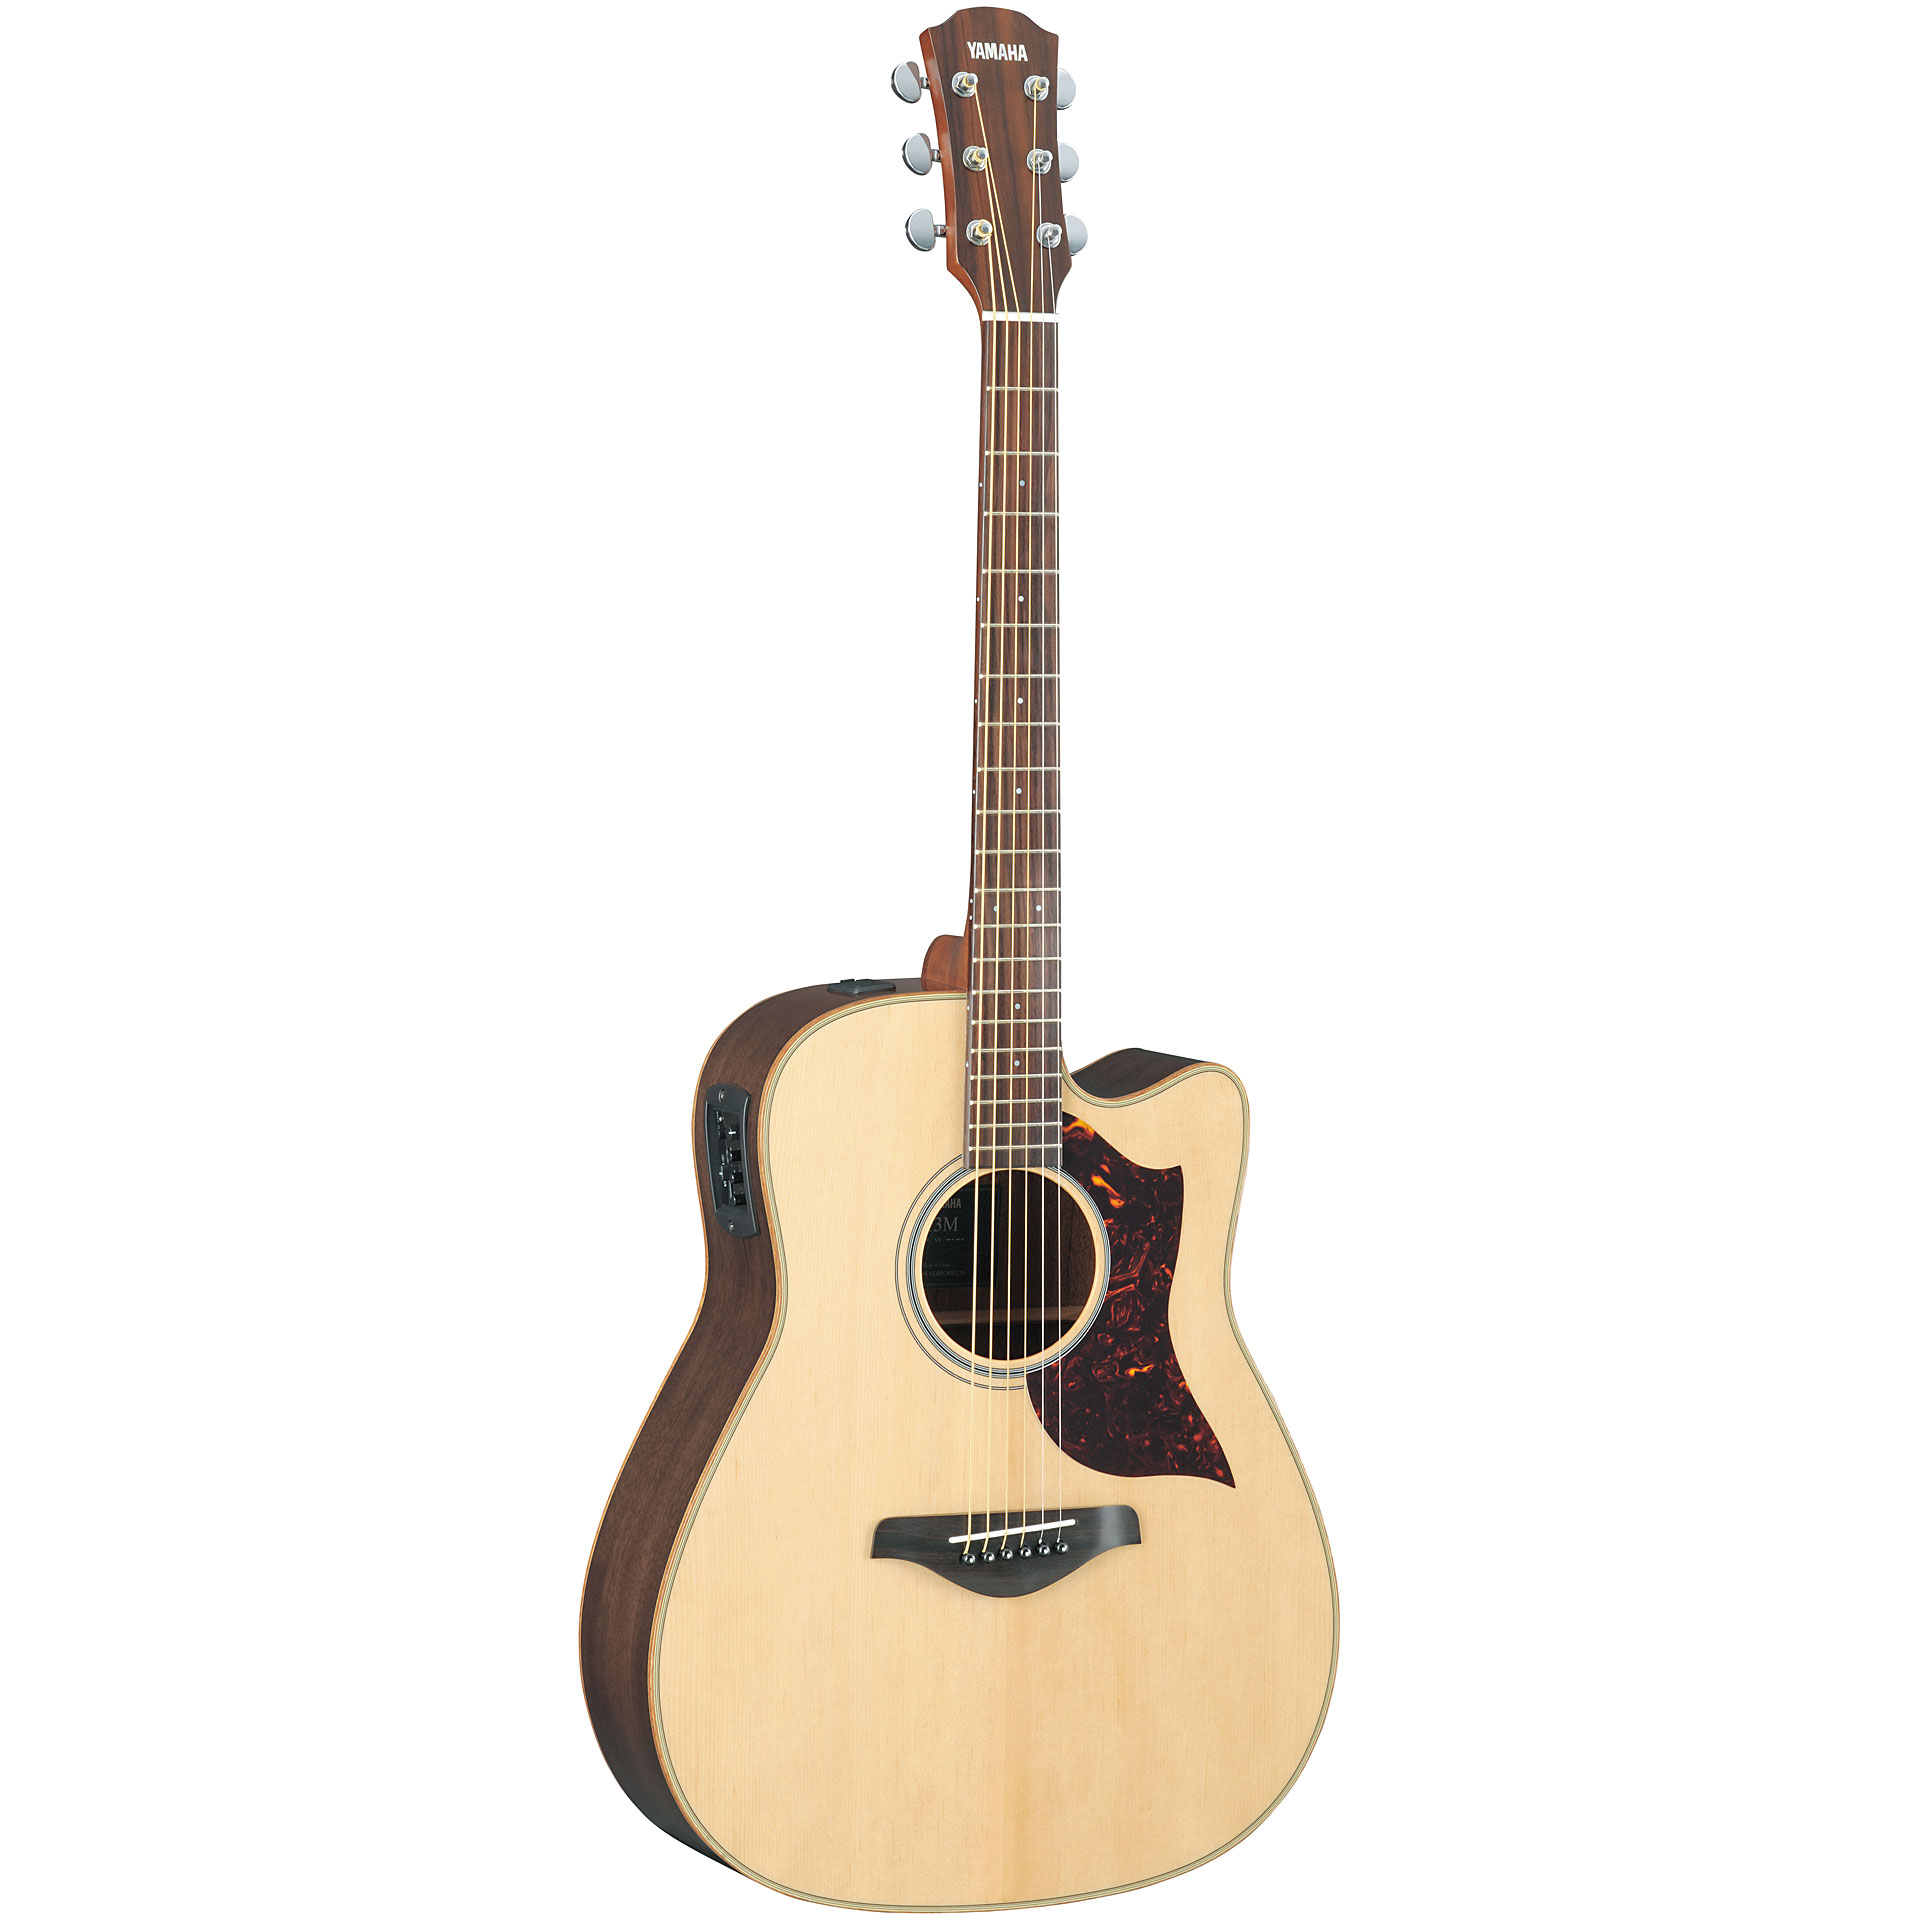
\includegraphics[width=4cm]{pictures/westerngitarre} &
    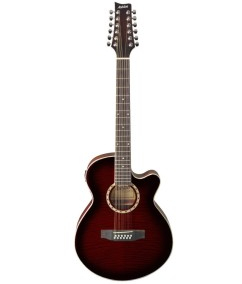
\includegraphics[width=3.75cm]{pictures/12saitige} &
    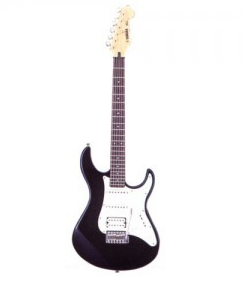
\includegraphics[width=3.75cm]{pictures/strat} &
    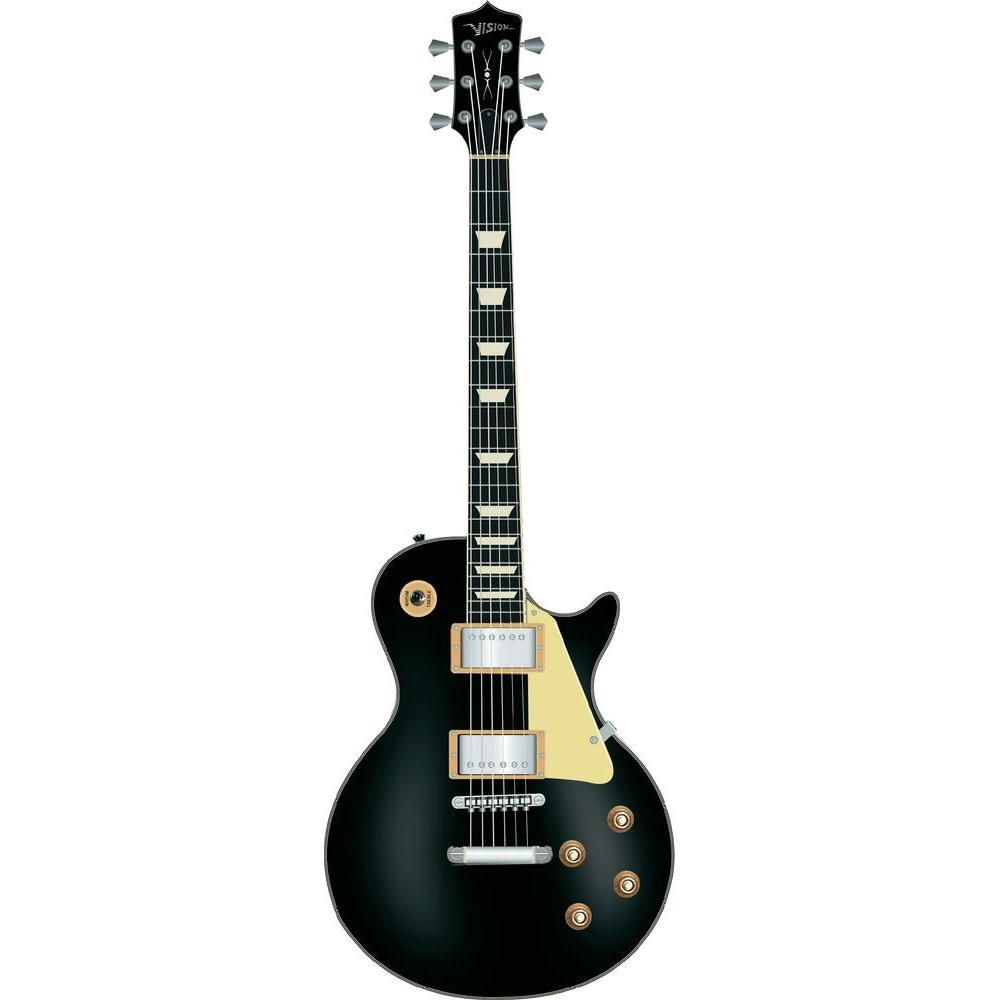
\includegraphics[width=4cm]{pictures/lespaul}\\
    Westerngitarre & 12 saitige Gitarre & E-Gitarre Typ Stratocaster & E-Gitarre Typ Les Paul
    \end{tabularx}
 

    \subsection{Aufbau}
    Der Aufbau der Konzertgitarre unterscheidet sich kaum vom Aufbau der oben gezeigten Gitarren und ist in \figref{fig:aufbau} dargestellt.
    \addImage{h}{width=0.8\textwidth}{pictures/guitar_labeled}{Der Aufbau der Gitarre}{fig:aufbau}
    \begin{itemize}
        \item \textbf{Die Wirbel} dienen zum Stimmen der Gitarre. Anhand des Widerstands beim Drehen ist einfach zu unterscheiden
        in welche Richtung beim Stimmen gedreht werden muss. Die Richtung, in der das Drehen leichter fällt stimmt die Saite tiefer.
        Andersherum wird der Ton der Saite höher gestimmt.
        \item \textbf{Der Sattel} dient dazu, die Saiten im \quotes{0. Bund} einheitlich am Griffbrett zu fixieren, was dazu führt, dass die sog. 
        leeren Saiten (Klang der Gitarre ohne irgendetwas am Griffbrett zu drücken) definierte Töne haben.
        \item \textbf{Ein Bundstab} erfüllt die gleiche Aufgabe wie der Sattel im \quotes{0. Bund} in den höheren Bünden. Der Abstand zwischen Sattel 
        und erstem Bundstäbchen wird als 1. Bund bezeichnet, der Abstand zwischen erstem und zweitem Bundstäbchen als zweiter Bund usw..
        \item \textbf{Das Griffbrett} enthält alle Bundstäbchen und wird später der Ort, an dem die linke Hand einzelne (oder mehrere) Töne greift.
        \item \textbf{Die Decke} der Gitarre schließt außer dem Schalloch den Korpus. Für manche Lieder kann sie zum erzeugen von Klopfrhythmen
        genutzt werden, indem mit der flachen Hand darauf geklopft wird.
        \item \textbf{Am Steg} werden die Saiten befestigt.
        \item \textbf{Die Saiten} sind wichtigster Bestandteil der Gitarre, da sie die Töne erzeugen.
    \end{itemize}

    \subsection{Saiten}
    Verschiedene Gitarrentypen haben verschiedene Saiten. Im Normalfall hat unsere Konzertgitarre 6 Naylonsaiten.
    In Ausnahmefällen können Konzertgitarren mit Stahlsaiten bespannt werden, sind meist aber nicht auf die höhere Spannung ausgelegt.
    Andere Gitarrentypen wie E- oder Westerngitarren verwenden Stahlsaiten, die metallische Klangeigenschaften haben und lauter klingen, als Nylonsaiten.

    Die Saiten werden in Bass- und Melodiesaiten unterteilt. Die tieferen drei Saiten, meist silber- oder goldfarben stellen die Ummantelten Basssaiten dar.
    Im Gegensatz zu den milchig durchsichtigen Melodiesaiten klingen sie tief.

    Für die normale Standardstimmung der Gitarre gibt es viele Merksprüche.
    Einer davon lautet:
    \begin{center}
    \large \textbf{E}\textcolor{black!50}{ine} \textbf{A}\textcolor{black!50}{lte} \textbf{D}\textcolor{black!50}{ame} \textbf{G}\textcolor{black!50}{eht} \textbf{H}\textcolor{black!50}{eute} \textbf{E}\textcolor{black!50}{inkaufen}
    \end{center}

    \subsection{Töne}
    \figref{fig:griffbrett} zeigt die Töne der Gitarre auf dem Griffbrett in Standardstimmung. Die dort farblich markierten Töne sind jeweils die selben. Es ist also dem Gitarrenspieler überlassen ob ein a auf dem 5. Bund der E- oder auf der leeren A-Saite gespielt wird.
    Die Zuordnung zwischen Noten und den Tönen auf dem Griffbrett zeigt \figref{fig:klaviatur}.
    In \figref{fig:griffbrett} sind zur der Übersichtlichkeit halber nur die Töne der C-Dur Tonleiter dargestellt, also nur die weißen Tasten des Klaviers.
    Wie auch das Klavier sind die Tonabstände der Gitarre zwischen den einzelnen Bünden Halbtöne.
    Die C-Dur Tonleiter besteht aus Ganztönen, weshalb im Regelfall immer ein Bund zwischen einzelnen Tönen ausgelassen wird.
    Die Ausnahmen stellen \textbf{\textcolor{black!50}{H und C}} und \textbf{\textcolor{black!50}{E und F}} dar, zwischen denen auch auf dem Klavier keine schwarze Taste existiert.
    Auf der Gitarre liegen diese Töne deshalb auf nebeneinander liegenden Bünden.
    \addImage{h}{width=0.6\textwidth}{pictures/tabulature.pdf}{Die Töne des Griffbretts}{fig:griffbrett}
    \addImage{h}{width=\textwidth}{pictures/klaviatur.pdf}{Tonleiter an der Kaviatur}{fig:klaviatur}

    \subsubsection*{Vorzeichen}
    In der Musik gibt es verschiedene Tonarten. Die einfachste und obig gezeigte ist die C-Dur Tonleiter.
    Sie ist deshalb gerade für Einsteiger geeignet, da sie vorzeichenfrei ist.
    Auf dem Klavier lässt sich dieser Begriff gut veranschaulichen, da nur die weißen Tasten verwendet werden.
    Die schwarzen Tasten stellen vorzeichenbehaftete Töne dar.

    \noindent Es wird zwischen zwei Arten von Vorzeichen unterschieden, die in \figref{fig:klaviatur} veranschaulicht sind.\\
    \textbf{Das \flat-Vorzeichen} vermindert einen Ton um einen Halbton. Das heißt aus einem g' würde ein ges', oder aus einem f'' ein e''.
    Der Name des verminderten Tons wird in der Regel mit einem angehängten '-es' gebildet.\\
    \newpage
    \noindent\textbf{Das \sharp-Vorzeichen} erhöht einen Ton um einen Halbton. Das heißt aus einem c' würde ein cis', oder aus einem e'' ein f''.
    Der Name des erhöhten Tons wird in der Regel mit einem angehängten '-is' gebildet.\\

    \subsection{Haltung}
    \subsubsection{Linke Hand}

    \subsubsection{Rechte Hand}

    \section{Das Zupfen}
    Beim Zupfen handelt es sich um eine Technik der rechten Hand. 

    \newpage
    \section{Bildquellen}
    Bei allen nicht aufgeführten Grafiken handelt es sich um selbst erstellte oder sehr stark modifizierte Grafiken.\vspace{0.5cm}\\
    \begin{tabularx}{\textwidth}{llX}
        \textbf{Seite} & \textbf{Name} & \textbf{URL} \\
        Titel & Gitarre & \small \url{http://wallpaper-gallery.net/single/guitar-wallpaper/guitar-wallpaper-10.html}\\
        1 & Westerngitarre & \small \url{https://www.musik-produktiv.de/yamaha-a1r.html}\\
        1 & Stratocaster & \small \url{http://msug.ch/instrumente/e-gitarre} \\
        1 & Les Paul & \small \url{https://www.conrad.at/de/lsc-2-e-gitarre-302488.html} \\
        1 & 12 saitige Gitarre & \small \url{http://gitarre-kaufen.net/12-saitige-gitarre} \\
        1 & Aufbau der Gitarre & \small \url{https://de.wikipedia.org/wiki/Gitarre} \\
    \end{tabularx}

\end{document}